% This is a LaTeX template for a submission to American Journal of Political Science
% If you find any errors, please let me know: jjharden@unc.edu
\documentclass[12pt, letterpaper]{article}
 
%==============Packages & Commands=================
\usepackage{graphicx} % Graphics
\usepackage{indentfirst} % Tells LaTeX to indent every paragraph 
\usepackage{setspace} % To set line spacing
\usepackage[longnamesfirst]{natbib} % For references
\usepackage{booktabs} % For tables
\usepackage{rotating} % For sideways tables/figures
\usepackage{amsmath} % Some math symbols
\usepackage[margin = 1in]{geometry}
\usepackage{subfig}
\usepackage{mdwlist}
\usepackage{url}
\usepackage{verbatim}
\urlstyle{same}
\usepackage{multirow}
\usepackage[nolists]{endfloat} % Figures and tables at the end
\newcommand{\R}{\texttt{R}\space} % Write R in typewriter font
\newcommand{\trans}[1]{{#1}^{\ensuremath{\mathsf{T}}}} % Transpose symbol 
\bibpunct{(}{)}{;}{a}{}{,} % Reference punctuation 
\captionsetup[subfloat]{position = top, font = large} % For sub-figure captions

%===============Some new commands==================
\newcommand{\fnote}[1]{\footnote{\begin{doublespace}\normalsize{#1}\vspace{-26pt}\end{doublespace}}} % 12 pt, double spaced footnotes 
\renewcommand{\figureplace}{ % This places [Insert Table X here] and [Insert Figure Y here] in the text
\begin{center}
[Insert \figurename~\thepostfig\ here]
\end{center}}
\renewcommand{\tableplace}{%
\begin{center}
[Insert \tablename~\theposttbl\ here]
\end{center}}

%============Article Title, Authors================
\title{The title}
\author{Your name\thanks{Acknowledgements}}

%===================Startup========================
\begin{document} 
\maketitle
\doublespacing
\vspace{5.5in}
\noindent Note: Note on replication data.
\thispagestyle{empty}
%===================Abstract======================= 
\newpage
\thispagestyle{empty}
\begin{abstract}
\begin{normalsize}
\noindent Abstract goes here.

\end{normalsize}
\end{abstract}

\begin{quote}
\textbf{Keywords}: Keywords go here.
\end{quote}
%================Begin Manuscript==================
\newpage
Internet speeds have increased dramatically over time (See Figure \ref{fig:speed_cbsa}, which plots speed separately by CBSA). In 2008, the average download speed in the United States was roughly 5.8 megabytes per minute; by 2014 the average speed was roughly 4 times faster--20 times faster. MORE

\begin{figure}
\centering
\caption{Average Download Speed by Core Base Statistical Area, 2008-2014}
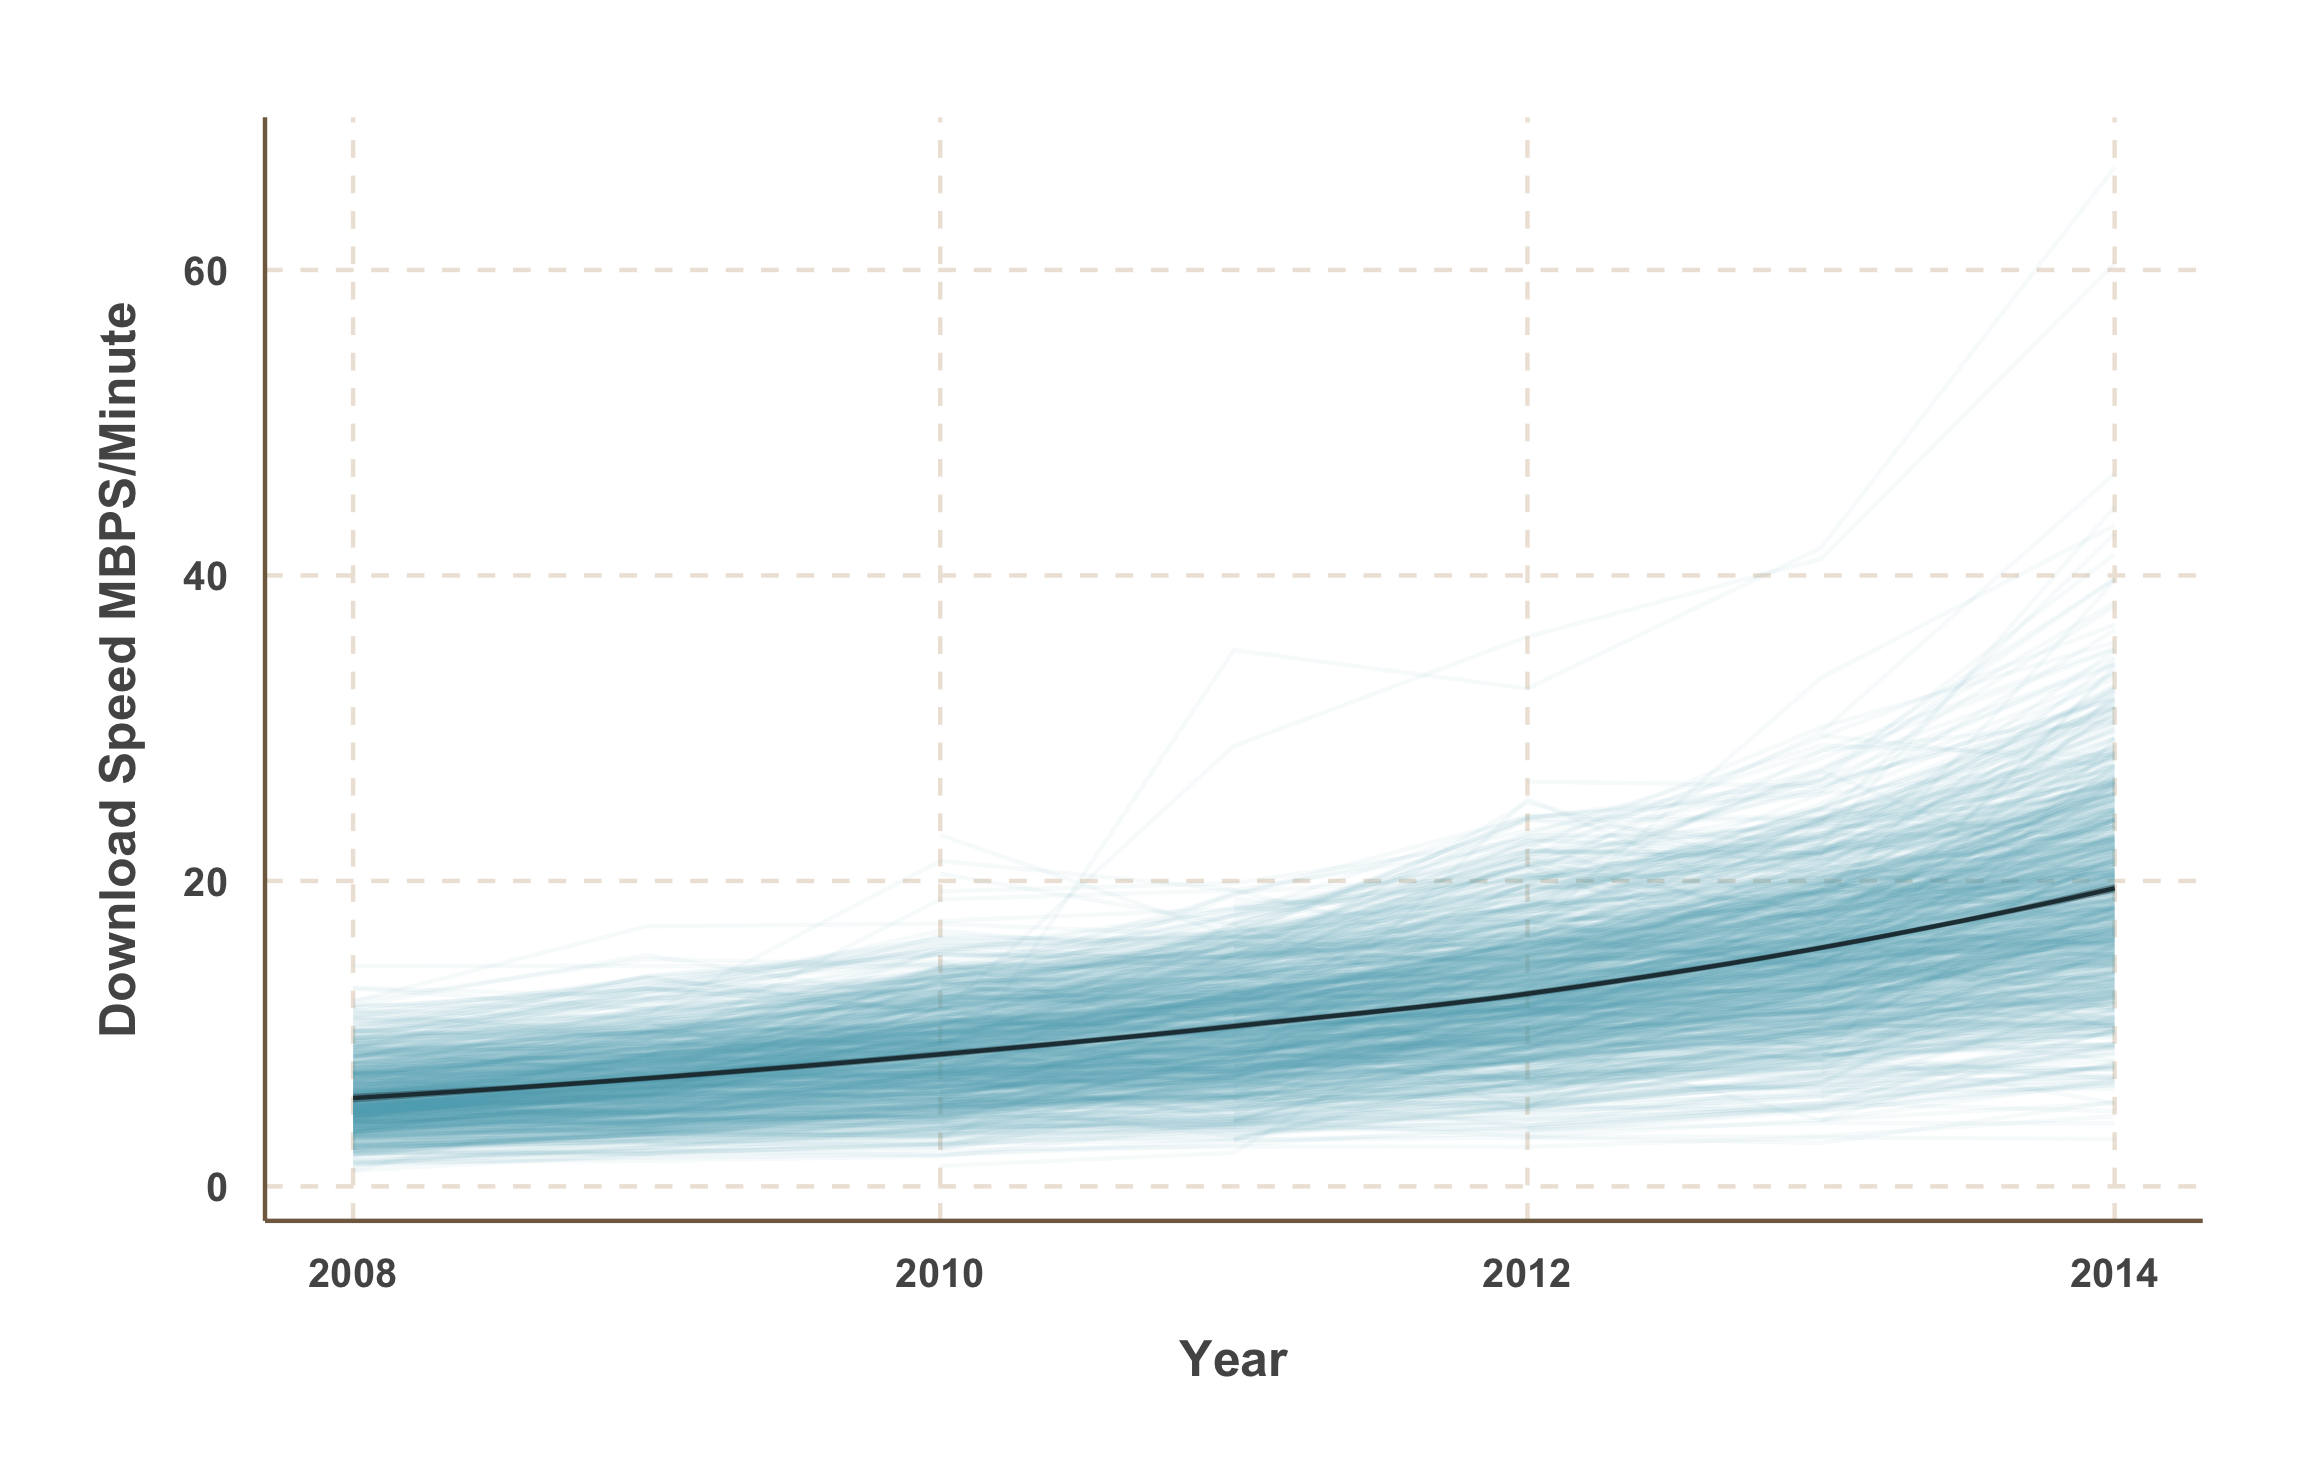
\includegraphics[width=\textwidth]{Graphs/speed_by_cbsa}
\label{fig:speed_cbsa}
\end{figure}

However, there is substantial variance in the growth of Internet speeds between cities. The fit of a model one with a fixed-effect for year and a random intercept nested within CBSA is significantly worse than the fit of a model with both a random intercept and slope nested within CBSA (AIC is 576.26 versus -664.58, respectively ,$\Chi$^2(2)=1244.8. p<.001)



%===================References=====================
\newpage
\bibliographystyle{apsr}
\bibliography{Name of your .bib file}

%===================End Document===================
\end{document}


